\documentclass{standalone}

\usepackage[dvipsnames]{xcolor}
\usepackage{tikz}
\usepackage{verbatim}
\usetikzlibrary{calc,trees,positioning,arrows,chains,shapes.geometric,%
    decorations.pathreplacing,decorations.pathmorphing,shapes,%
    matrix,shapes.symbols, plotmarks}

 \begin{document}
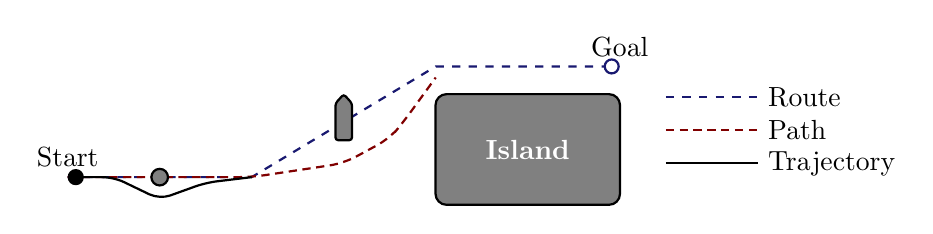
\begin{tikzpicture}[x=6.65em,y=4em]

	\tikzstyle{block} = [rectangle, draw, thick,
    		text width=6em, text centered, rounded corners, minimum height=4em]
	\tikzstyle{block_marked} = [block, fill=MidnightBlue, text=white, font=\bfseries]
	\tikzstyle{plaintext} = [draw=none,fill=none,text width=6em, text centered]
	\tikzstyle{line} = [draw, ->,>=stealth, thick, rounded corners]

   
    
    \draw [thick,dashed,MidnightBlue,-o]
		(-2,0) node[anchor=south,black]{Start} -- (-1,0) -- (0,1) -- (1,1)  node[anchor=south,black]{Goal} ;
		
	\draw [thick, densely dashed, Maroon,rounded corners=5]
		(-2,0) -- (-1,0) -- (-0.5,0.125) -- (-0.25,.35) -- (-0.175,0.5) -- (0,.9);
		
	\draw [thick, black,rounded corners, *-]
		(-2,0) -- (-1.75,0) -- (-1.5,-0.2) -- (-1.25,-.05) -- (-1,-0);
		
	\node[block,fill=gray,text=white,font=\bfseries] at (0.5,0.25) {Island};
	
	\draw [thick,fill=gray] (-1.5,0) circle (3pt);
	

  	
  	\begin{scope}[shift={(-0.5,0.5)},scale=.1, rotate=90, rounded corners=1, thick] 
		\draw[fill=gray] (-1,-.75) -- (1,-.75) -- (1.5,0) -- (1,.75) -- (-1,.75) -- cycle;
  	\end{scope} 
		
		
		%legend
	\begin{scope}[shift={(1.25,0.125)}] 
		\draw [thick,black] (0,0) -- (0.5,0) 
		node[right]{Trajectory};
		\draw [yshift=\baselineskip, thick,densely dashed,Maroon] (0,0) -- (0.5,0) 
		node[right,black]{Path};
		\draw [yshift=2\baselineskip, thick,dashed,MidnightBlue] (0,0) -- (0.5,0) 
		node[right,black]{Route};
	\end{scope}
\end{tikzpicture}
\end{document}